\mySection{Experimental Settings}
In this section, we assess the practicality of PyRollCall. Two of the most important
functionalities of a facial recognition roll call system are: (1) face detection
and (2) facial recognition. If these two features work accurately, then the system
is considered to be working as intended. Firstly, we evaluate the performance of face detection.
Figure~\ref{fig:face-detection-test} shows that PyRollCall is able to detect all faces
within the image regardless of head tilt, rotation and even facial expressions.
\vspace{0.2cm}

\begin{figure}[!htb]
  \centering
  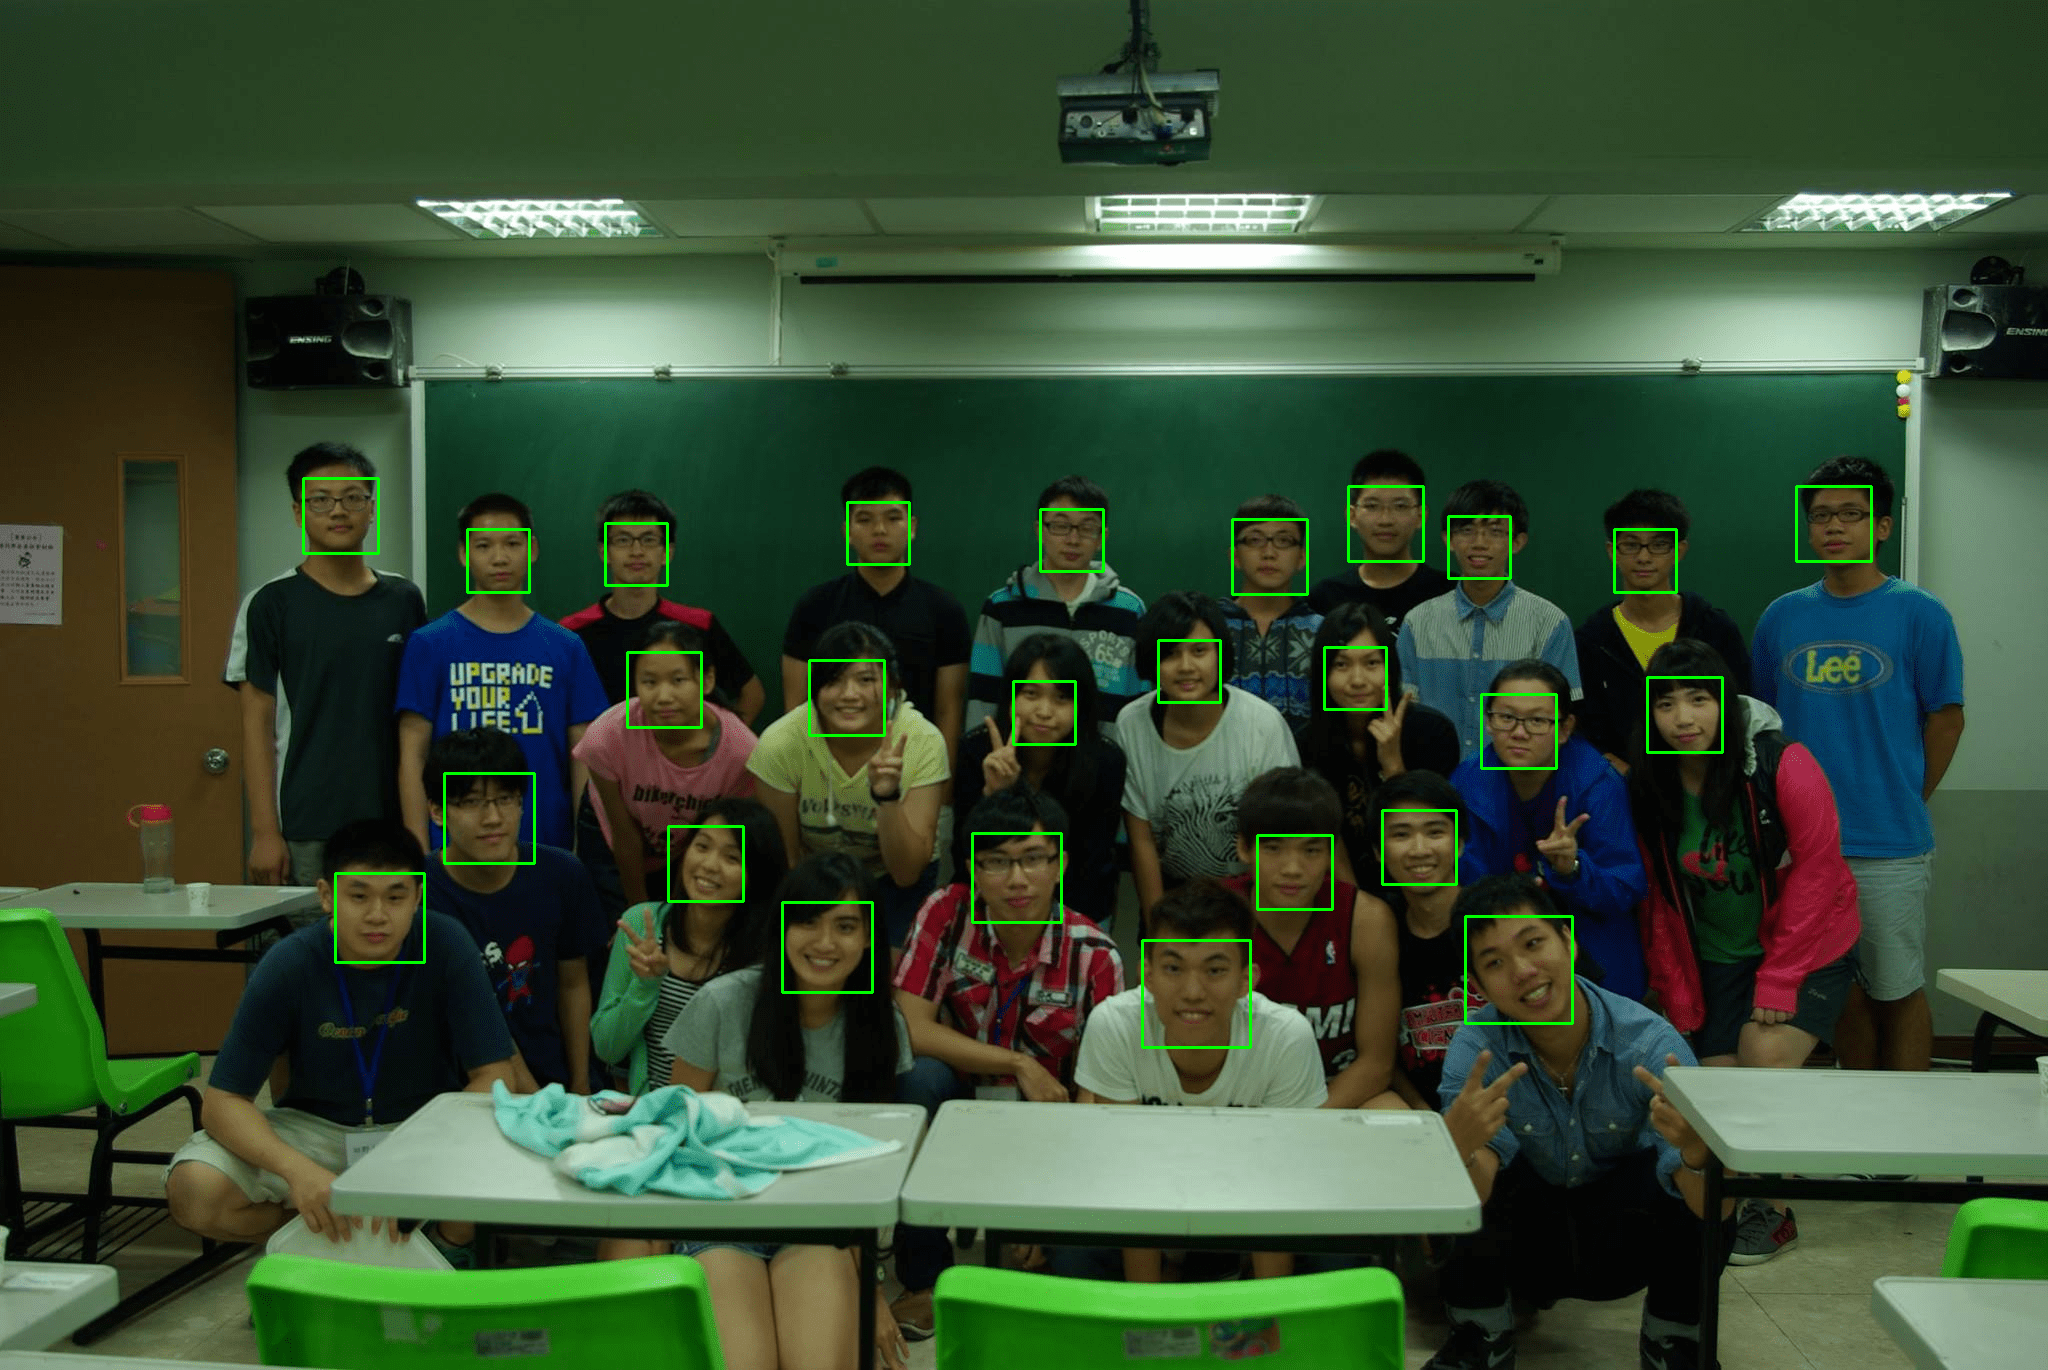
\includegraphics[height=8.5cm]{figures/face-detection-test.png}
  \caption{Face Detection}
  \label{fig:face-detection-test}
\end{figure}

In our experiments, all faces are facing upfront to the camera, and thus the successful
rate of face detection is rather high. In real-world scenarios, the faces of students
may be turned into various angles and the results of face detection will vary. Hence,
when taking photos from the students, the teacher will have to ask for the attention from
the students for a few seconds.
\vspace{0.5cm}

Secondly, we evaluate the effectiveness of facial recognition. Figure~\ref{fig:facial-recog-test}
demonstrates a successful facial recognition performed by PyRollCall. In order to make
the facial recognition feature works correctly, the teacher should collect 10 to 15 photos
(or ideally 15 to 25 photos) from each student and let PyRollCall pre-compute all of the
facial embeddings from each photo.
\vspace{0.5cm}

\begin{figure}[!htb]
  \centering
  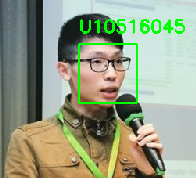
\includegraphics[]{figures/facial-recog-test.png}
  \caption{Facial Recognition}
  \label{fig:facial-recog-test}
\end{figure}
